\section{La categoría AutoModelCar}

\begin{frame}\frametitle{La categoría AutoModelCar}
  \begin{itemize}
  \item Se originó por el proyecto \textit{Visiones de movilidad urbana} a través del cual se donaron vehículos a escala a varias instituciones educativas y de investigación del país
    \begin{figure}
      \centering
      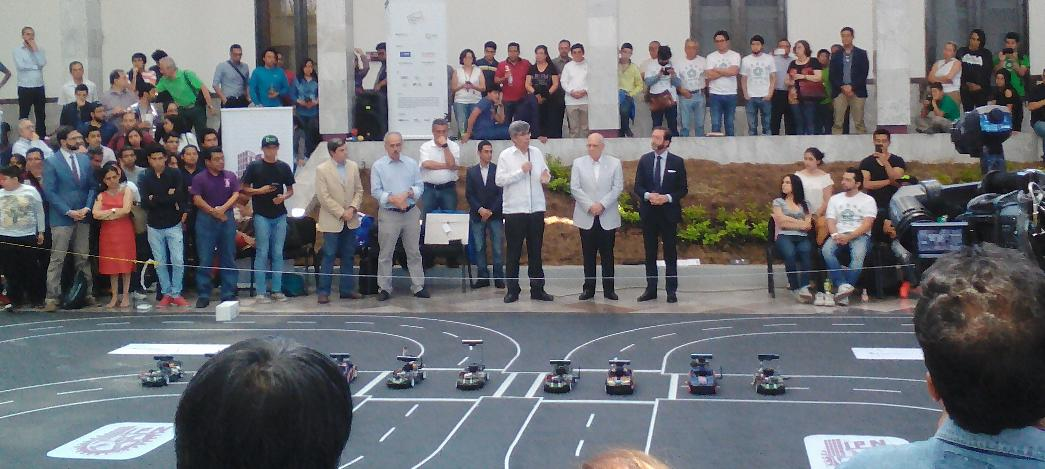
\includegraphics[width=0.9\textwidth]{Figuras/VisionesDeMovilidadUrbana.jpg}
    \end{figure}
  \end{itemize}
\end{frame}

\begin{frame}\frametitle{La categoría AutoModelCar}
  \begin{itemize}
  \item Originalmente solo se permitían vehículos AutoNOMOS:
    \begin{figure}
      \centering
      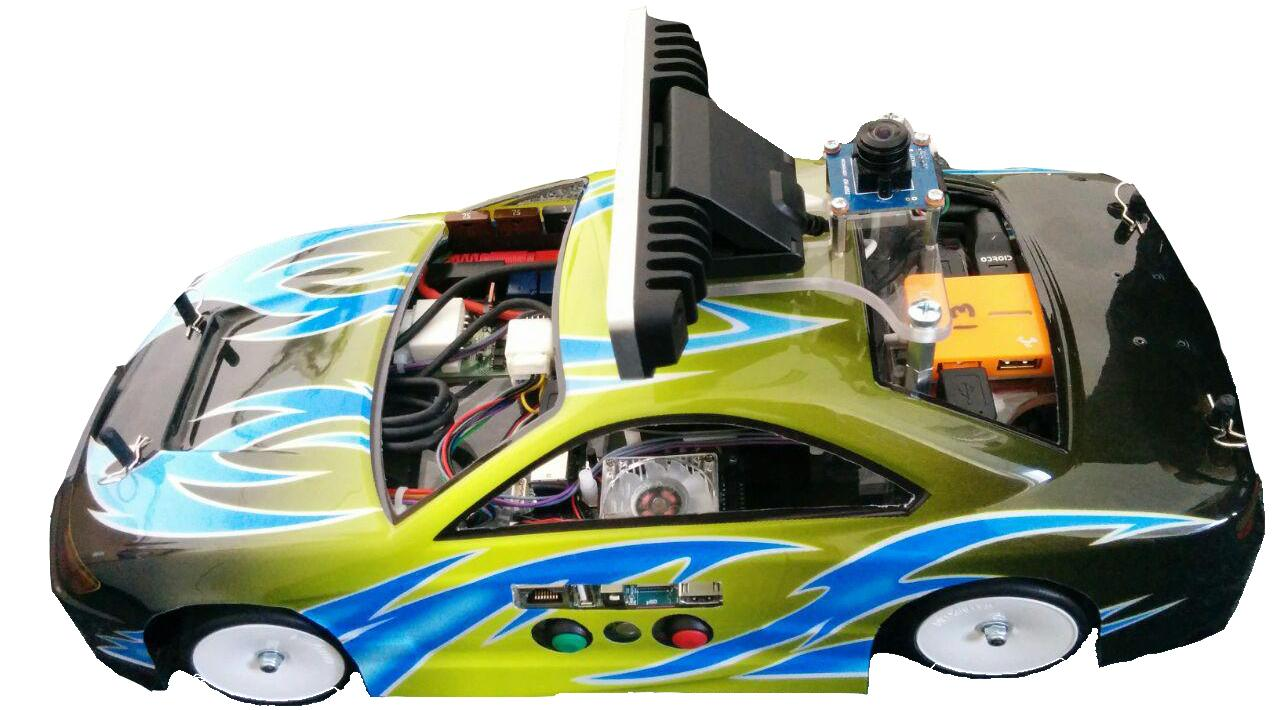
\includegraphics[width=0.35\textwidth]{Figuras/AutoNOMOS.jpg}
    \end{figure}
  \item Pero ahora se puede participar con cualquier vehículo a escala:
    \begin{figure}
      \centering
      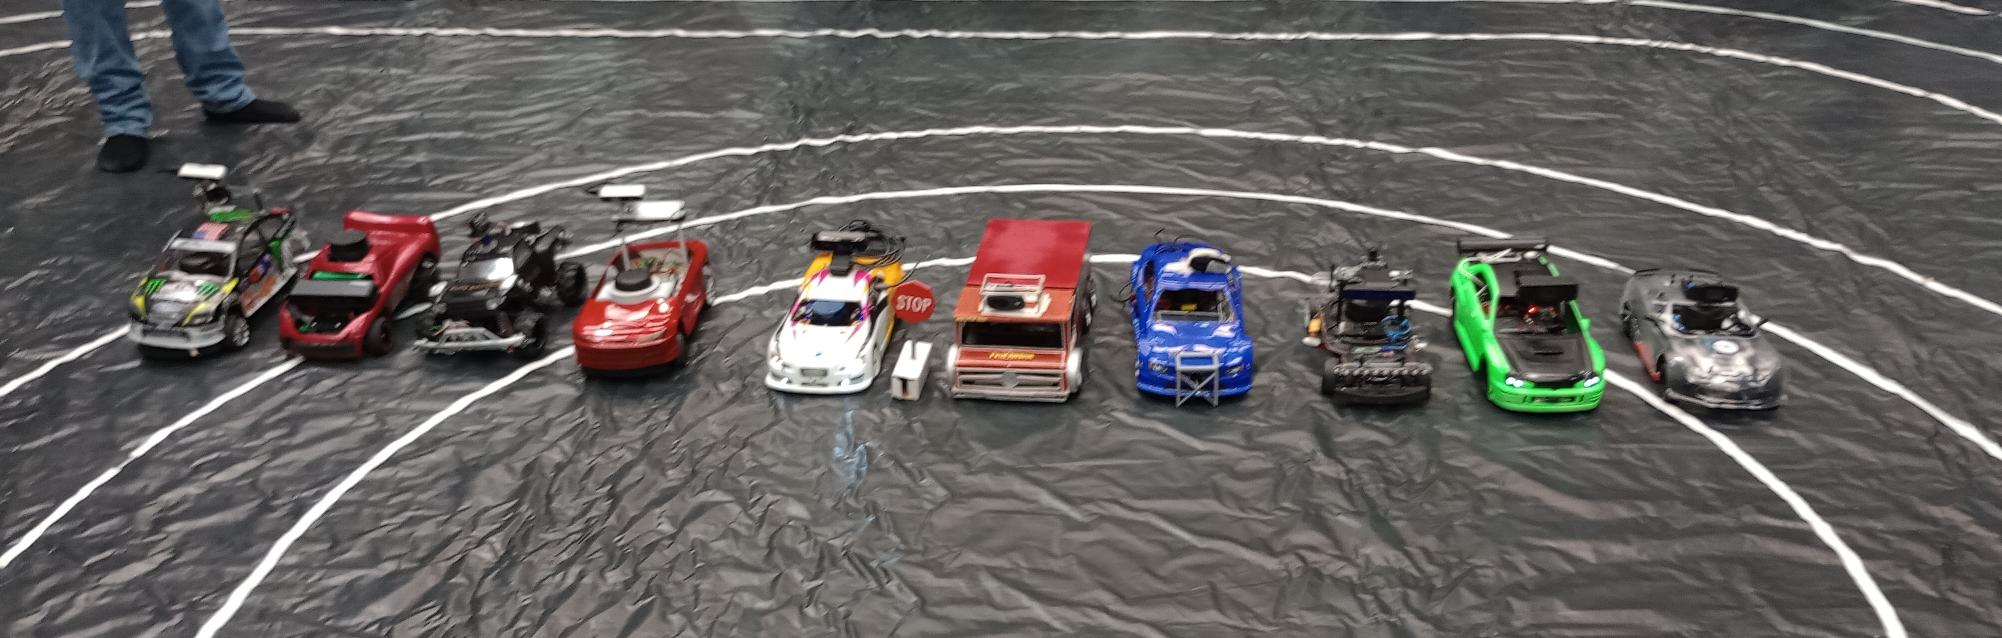
\includegraphics[width=0.75\textwidth]{Figuras/AutoModelCarCars.jpg}
    \end{figure}
  \end{itemize}
\end{frame}

\begin{frame}\frametitle{La categoría AutoModelCar}
  \begin{itemize}
  \item La competencia consta de cuatro pruebas (esperemos aumentarlas este año):
    \begin{multicols}{2}
      \begin{itemize}
      \item Navegación autónoma sin obstáculos
      \item Navegación con obstáculos estáticos
      \item Navegación con obstáculos en movimiento
      \item Estacionamiento
      \end{itemize}
    \end{multicols}
    \begin{figure}
      \centering
      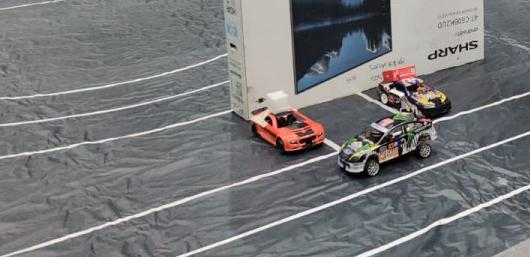
\includegraphics[width=0.6\textwidth]{Figuras/AutoModelCarEstacionamiento.jpg}
    \end{figure}
  \end{itemize}
\end{frame}

\begin{frame}\frametitle{La categoría AutoModelCar}
  Se utiliza una pista con rectas, curvas y cruces:
  \begin{figure}
    \centering
    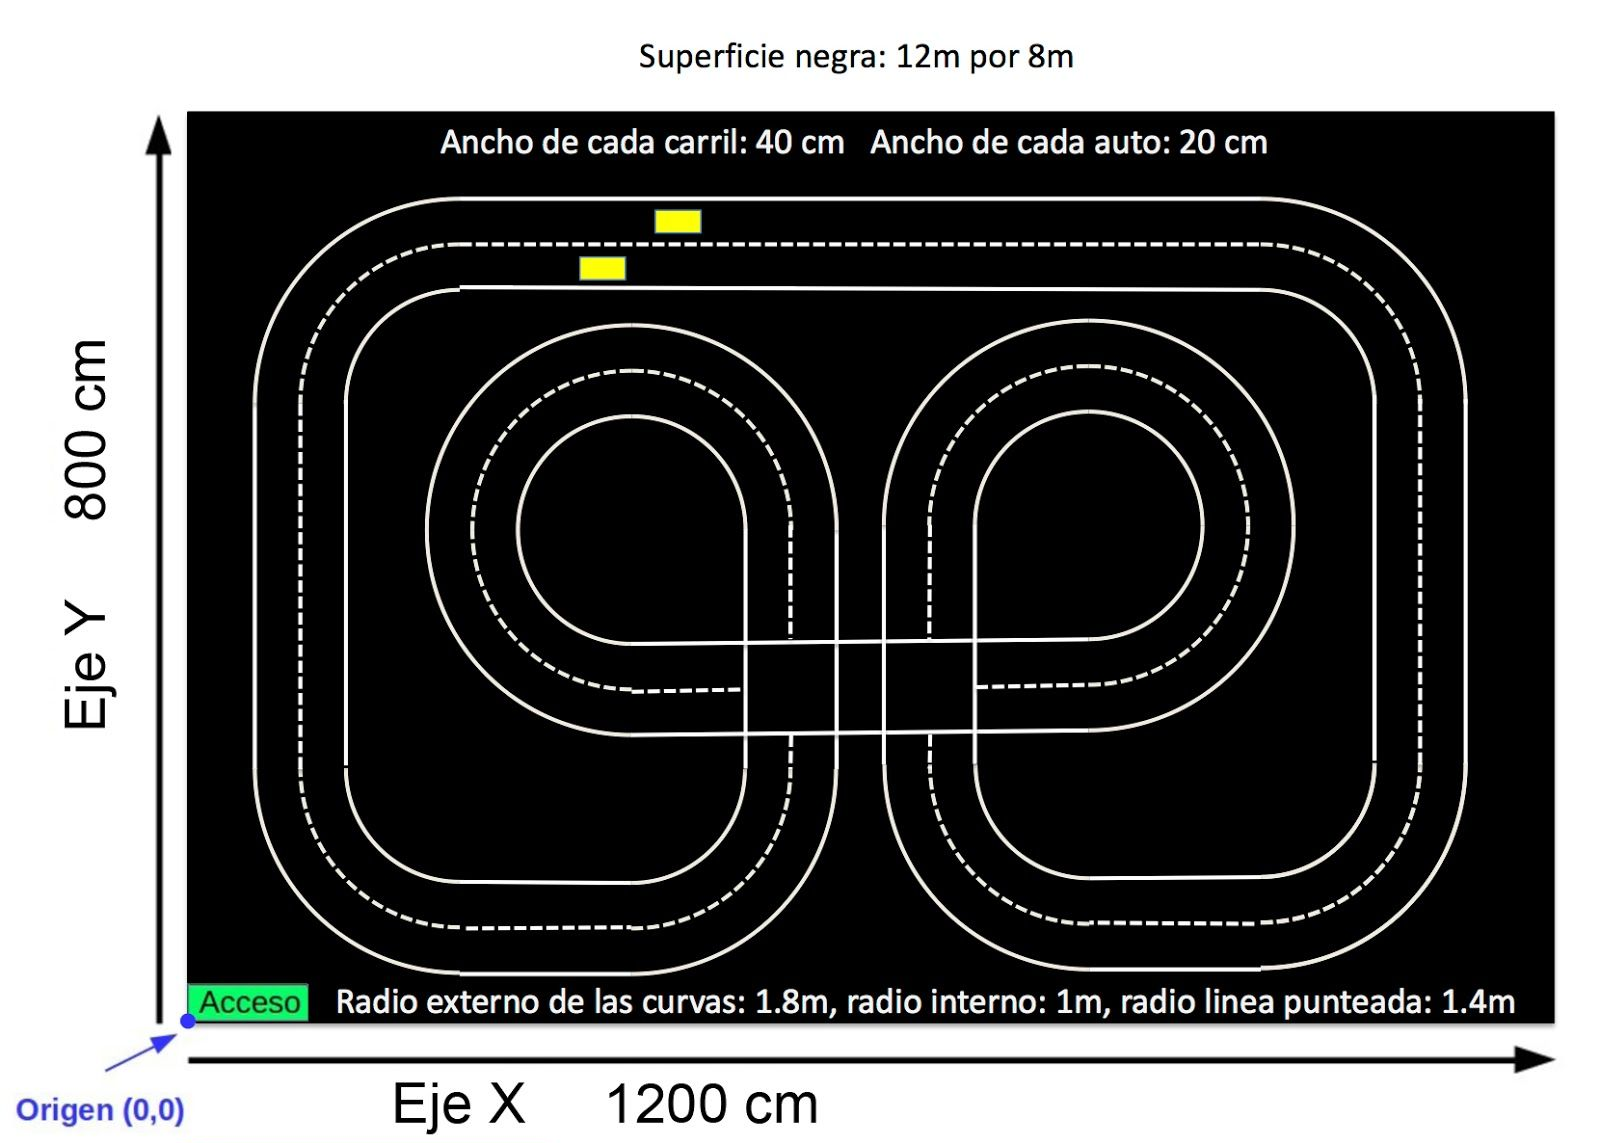
\includegraphics[width=0.7\textwidth]{Figuras/AutoModelCarPista.png}
  \end{figure}
\end{frame}

\begin{frame}\frametitle{Hardware para vehículos sin conductor}
  \begin{figure}
    \centering
    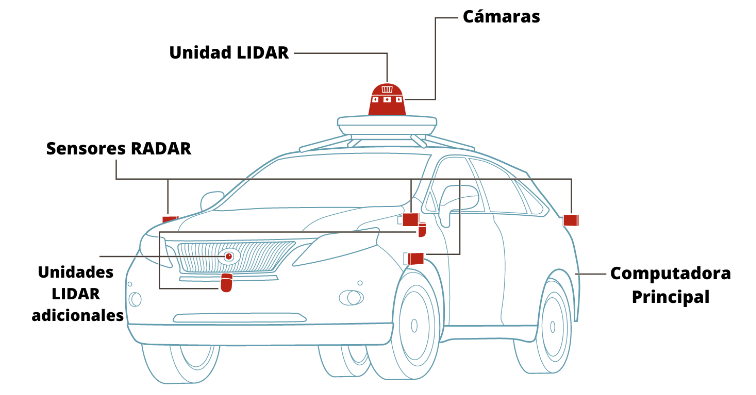
\includegraphics[width=0.6\textwidth]{Figuras/Hardware.png}
  \end{figure}
\end{frame}

\begin{frame}\frametitle{Herramientas de simulación}
  ¿Por qué utilizar simuladores?
  \begin{itemize}
  \item Instrumentar un vehículo autónomo puede ser costoso, incluso si se hace a escala.
  \item En simulación se pueden construir ambientes controlados que permiten probar partes específicas del sistema de autonomía.
  \item Se pueden enfocar los esfuerzos al desarrollo de software dando por hecho un hardware funcional.
  \item Algunos ejemplos de simuladores:
    \begin{itemize}
    \item Gazebo (utilizado en el TMR 2021)
    \item Webots (utilizado en los TMRs 2022 y 2023)
    \item Matlab (utilizado por quien tiene dinero para pagar la licencia)
    \end{itemize}
  \end{itemize}
\end{frame}

\begin{frame}\frametitle{El simulador Webots}
  El simulador Webots tiene varias características para simulación de vehículos sin conductor:
  \begin{itemize}
  \item Motor de físicas ODE y OpenGL como motor de renderizado.
  \item Multiplataforma y disponible para sistemas operativos Linux, Windows y macOS.
  \item Programación en diferentes lenguajes: C, C++, Python, Java, MATLAB.
  \item Amplía variedad de robots, sensores, actuadores, objetos y materiales.
  \item Fácil integración con la plataforma ROS.
  \end{itemize}
  \begin{figure}
    \centering
    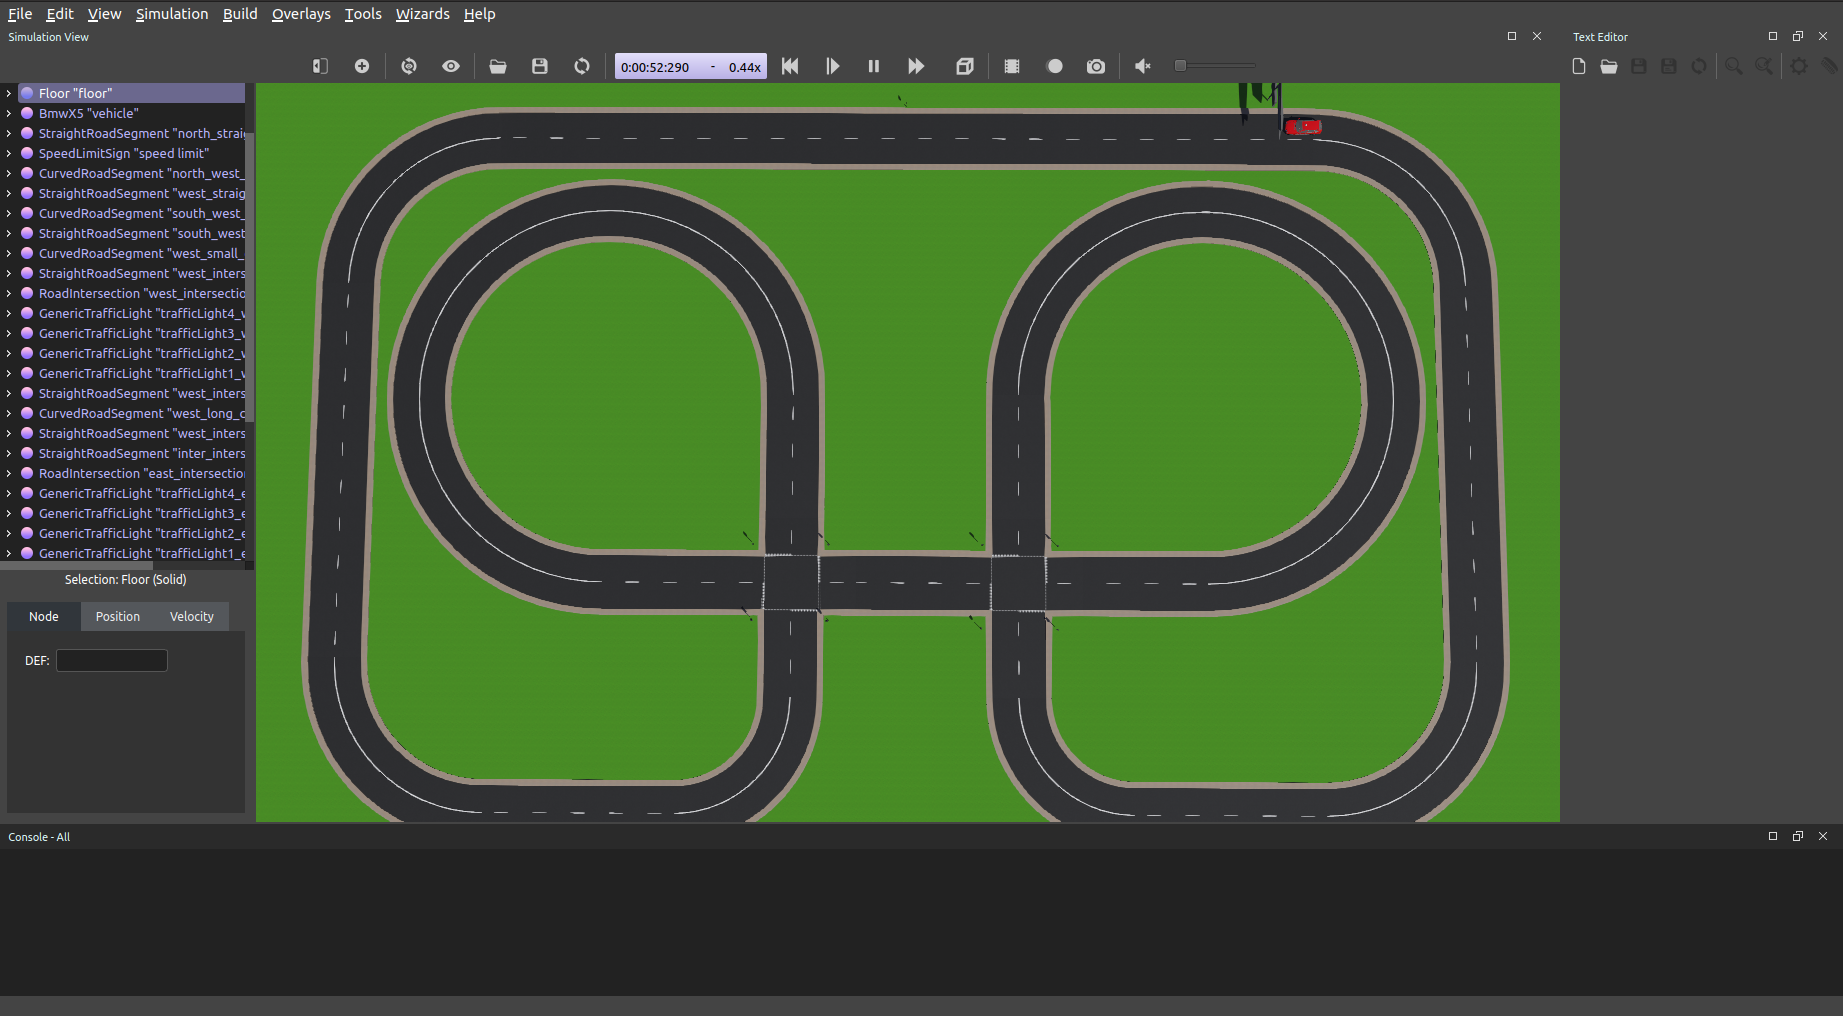
\includegraphics[width=0.7\textwidth]{Figuras/WebotsExample.png}
  \end{figure}
\end{frame}

\begin{frame}\frametitle{SUMO (Simulation of Urban Mobility)}
  Es un paquete de simulación de tráfico desarrollado por el Centro Aeroespacial Alemán.
  \begin{itemize}
  \item De código abierto
  \item Diseñado para manejar redes grandes de vehículos
  \item Se pueden simular vehículos, peatones, ciclistas, señales de tránsito, transporte público, entre muchas otras opciones
  \item Fácil intregración con Webots mediante el objeto \textit{SUMO interface}:
  \item Se puede definir el comportamiento de los vehículos mediante archivos \texttt{*.nod.xml}, \texttt{*.edg.xml}, \texttt{*.net.xml}, \texttt{*.rou.xml} y \texttt{*.sumocfg}
  \end{itemize}
\end{frame}

\begin{frame}[containsverbatim]\frametitle{Ejercicio 1 - Herramientas de simulación}
  \begin{enumerate}
  \item Abra una terminal y ejecute la simulación con el comando:
    \begin{lstlisting}[language=bash,numbers=none]
roslaunch eir2024 navigation_moving_obstacles.launch
    \end{lstlisting}
  \item Detenga la simulación
  \item Abra el archivo \texttt{catkin\_ws/src/eir2024/worlds/navigation\_moving\_obstacles\_net/sumo.rou.xml} y descomente las líneas 8 a 14
  \item Corra nuevamente la simulación. Se deberían observar más vehículos
  \item Detenga la simulación y ejecute los siguientes comandos:
    \begin{lstlisting}[language=bash,numbers=none]
roscd eir2024/worlds/navigation_moving_obstacles_net/
netconvert -S 10 -n sumo.nod.xml -e sumo.edg.xml -o sumo.net.xml
    \end{lstlisting}
  \item Corra nuevamente la simulación. Se debería notar un cambio en la velocidad de los vehículos
  \end{enumerate}
\end{frame}
